\documentclass[12pt,a4paper]{article}

\usepackage[english]{babel}
\usepackage{amsmath}
\usepackage{upgreek}
\usepackage{paralist}

\newcommand{\A}{\mathcal{A}}
\newcommand{\OC}{\mathcal{O}}
\newcommand{\V}{\mathcal{V}}
\newcommand{\G}{\mathcal{G}}
% OSTblock
\newcommand{\B}{\mathcal{B}}
\newcommand{\BS}{\operatorname{BS}}
\newcommand{\BE}{\operatorname{BE}}
% State root
\newcommand{\SR}{\operatorname{SR}}
% Storage root
\newcommand{\SO}{\operatorname{SO}}
% OSTblock gas limit
\newcommand{\OL}{\operatorname{OL}}


% make in the latest NIPS format (as of this writing, 2017)

\usepackage[nonatbib,final]{nips_2017}
%\usepackage[nonatbib,final]{nips_2017}

\usepackage{color}
\usepackage{graphicx}
\DeclareGraphicsExtensions{.pdf,.eps,.png,.jpg}		% search for .pdf, then .eps, then .pngs, then .jpg

% look in these subdirectories for graphics referenced by \includegraphics
% each entry must end with a /
\graphicspath{{figs/}{figures/}{images/}{./}}

\newcommand*{\red}[1]{ \color{red} #1}

%\usepackage{tabularx}
\usepackage{url}
\usepackage{amsmath}

% this is for environments \subfigure and \subtable
\usepackage{subcaption}

% These packages are FORBIDDEN
%%%%%%%%%%%%%%%%%%%%%%%%%%%%%%%%%%%%%%%%%%%%%%%%%%%%%%%%
%\usepackage{lmodern} % messes up \textsc
%\usepackage{cite} % messes up NIPS
%\usepackage{fullpage} % messes up NIPS
%\usepackage{natbib} % messes up NIPS
%%%%%%%%%%%%%%%%%%%%%%%%%%%%%%%%%%%%%%%%%%%%%%%%%%%%%%%%

\usepackage{array}			% replacement for eqnarray.  Must be BEFORE \usepackage{arydshln}
\usepackage{units}			% for \nicefrac{\alpha}{\beta}


\usepackage{amsthm}		% for theorems
\newtheorem{definition}{Definition}

% text looks a little better
\usepackage{microtype}

\usepackage{wasysym}

\usepackage{textcomp, marvosym} % pretty symbols
\usepackage{booktabs} 	% for much better looking tables

% for indicator functions
\usepackage{dsfont}

% For automatic capitalizaton of section names, etc.
\usepackage{titlesec,titlecaps}


\Addlcwords{is with of the and in}
\Addlcwords{of the}
\Addlcwords{and}
\titleformat{\section}[block]{}{\normalfont\Large\bfseries\thesection.\;}{0pt}{\formatsectiontitle}
\newcommand{\formatsectiontitle}[1]{\normalfont\Large\bfseries\titlecap{#1}}

\titleformat{\subsection}[block]{}{\normalfont\large\bfseries\thesubsection.\;}{0pt}{\formatsubsectiontitle}
\newcommand{\formatsubsectiontitle}[1]{\normalfont\large\bfseries\titlecap{#1}}





% for pretty Euler script
% \usepackage[mathscr]{euscript}
% \usepackage{bold-extra}





%\usepackage{subfig}
\usepackage{float} % for \subfloat

%%%%%%%%%%%%%%%%%%%%%%%%%%%%%%%%%%%%%%%%%%
%% More customizable Lists
%%%%%%%%%%%%%%%%%%%%%%%%%%%%%%%%%%%%%%%%%%
% Better symbols custom enumerative lists, define any symbol you'd like
% \usepackage{enumitem}


%%%%%%%%%%%%%%%%%%%%%%%%%%%%%%%%%%%%%%%%%%
%% Custom Symbols 
%%%%%%%%%%%%%%%%%%%%%%%%%%%%%%%%%%%%%%%%%%
% \xspace at the end of custom macros never screws up spacing.
\usepackage{xspace}



%%%%%%%%%%%%%%%%%%%%%%%%%%%%%%%%%%%%%%%%
%% Abbreviations you'll always want
%%%%%%%%%%%%%%%%%%%%%%%%%%%%%%%%%%%%%%%%
\newcommand*{\TODO}[1]{{\centering {\small \sffamily \color{red} #1} \vskip10pt }}
\newcommand*{\todo}[1]{{\small \sffamily [{\color{red} #1}]}}
\newcommand*{\q}[1]{{\small \sffamily [{\color{blue} #1}]}}
\newcommand*{\fix}[1]{{\sffamily [{\textnormal{\color{red} #1}}]}}



%-----------------------------------------------------------------------------
%  Cross references
%-----------------------------------------------------------------------------
% The following code defines how you make references to figures, tables, etc...
% It is defined in one place only, and can be modified for all references
% in the document at the same time.
% Instead of typing each time: "see Fig. \ref{myfig}" you can create a command
% \figref which will do the job. Then in text you only type \figref{myfig} and LaTeX
% will do the rest.
\newcommand{\tblref}[1]{Table~\ref{#1}}
%\renewcommand*{\figref}[1]{Fig.~\ref{#1}}
\renewcommand{\eqref}[1]{eq.~(\ref{#1})}
\newcommand{\Subref}[1]{(\subref{#1})}


\newcommand{\figref}[1]{Figure~\ref{#1}}
\newcommand{\Figref}[1]{Figure~\ref{#1}}
\newtheorem{theorem}{Theorem}
\newtheorem{lemma}[theorem]{Lemma}

%%%%%%%%%%%%%%%%%%%%%%%%%%%%%%%%%%%%%%%%

% for \sout{} for strikeout
% \usepackage[normalem]{ulem}


% for better manipulation of tables
\usepackage{makecell}
\renewcommand\theadfont{\bfseries}


%-----------------------------------------------------------------------------
%  Misc symbols that I like
%-----------------------------------------------------------------------------
\newcommand*{\opname}[1]{\operatorname{#1}}


\renewcommand*{\to}{\rightarrow}


%%%%
\graphicspath{ {./images/} }

\title{OpenST\\\sc\Large{a framework for building token economies}}
\author{\textbf{Benjamin Bollen, Martin Schenck}\\ for OpenST Foundation}
\date{OpenST v0.10 - May 2018}

\begin{document}

\maketitle

\begin{abstract}
We present improvements to the OpenST protocol.
OpenST is a framework powered by Ethereum to build token economies.
We lay out in detail two contributions, OpenST Mosaic and OpenST Gateway,
which work together to scale Ethereum.
OpenST Mosaic is a layer-2
% TODO finish abstract
\end{abstract}

%
% Section
%
\section{Introduction}

%OpenST is a holistic solution powered by Ethereum to scale Ethereum to.

%
% Section
%
\section{OpenST}

\subsection{Use Cases}

\subsubsection{BT}

\subsubsection{DApp}

%
% Section
%
\section{Related Work}

\paragraph{Verifiers' Dilemma}
\cite{verifiersdilemma}

\paragraph{Interblockchain Communication}
\cite{cosmos}

\paragraph{Casper FFG}
\cite{casperffg}

%
% Section
%
\section{Our Contribution}

%
% Section
%
\section{Openly Scaling Blockchains}

\subsection{OpenST Gateway}
\label{subsec:gateway}

OpenST Gateway enables chain-to-chain transfer of state objects.

\subsection{OpenST Mosaic}
\label{subsec:mosaic}

OpenST Mosaic enables chain-to-chain state transfer.
That allows us to secure an insecure chain's state on a secure chain.
We call the secure chain \emph{origin} and the insecure one \emph{auxiliary}.
In order to be blockchain proposal mechanism agnostic, we layer Casper~\cite{casperffg} on top of both chains.

% TODO the following section is misplaced, not all concepts are known
In order to transfer and verify state, it is required to transfer state bi-directional between auxiliary and origin.
That way, auxiliary can verify that its state has been finalised on origin and
the set of validators, that is tracked on origin, is also known to auxiliary.

\emph{Validators} are actors that vote on state.
They are similar to validators in Casper~\cite{casperffg}.
Their deposit is stored on origin.
Similarly to Casper, their deposit rises and falls with rewards and penalties, respectively.
When we say "$\frac{2}{3}$ of validators", we equally refer to the deposit-weighted fraction.
However, there are different kinds of voting message types.
At this stage, we assume a fixed set of validators, $\V$.
A dynamic set of validators will be described later.

Validators can vote on a number of events:
\begin{inparaenum}[(a)]
	\item state transfers to auxiliary,
	\item checkpoint justifications on auxiliary, and
 	\item state transfers to origin.
\end{inparaenum}
When state is transferred from origin to auxiliary,
the validators vote according to the Casper rules like the state transfer represents a checkpoint.
On auxiliary, checkpoints are justified by supermajority links as described in Casper.
Casper applied to auxiliary the same way its application to Ethereum is described in the Casper paper.
When auxiliary's state is transferred to origin, a simple $\frac{2}{3}$ majority vote on that state commits it to origin.

% TODO explain alpha and OSTblock heights before defining the OSTblock header
\emph{OSTblocks} are a compressed representation of auxiliary's transactions.
% TODO are OSTblocks' transactions blocks or dynasties from auxiliary?
Transactions in an OSTblock each represent one block of the auxiliary chain.
An OSTblock transaction represents the state change from the beginning of its associated block to the end of that block.
The OSTblock header of block $\B_\alpha$ at height $\alpha$ contains:
\begin{enumerate}
	\item A link to the previous OSTblock
	\item The signatures of the validators in $\V_\alpha$
	\item The root hash of the state tree of auxiliary
	\item The set of validators for the next OSTblock, $\V_{\alpha+1}$
\end{enumerate}
We do not store the body of an OSTblock on origin, only the header.
The content can be re-created at any time from the auxiliary chain and proven with the state root.

% TODO process should be linked to figure fig:mosaic
% TODO extend process to describe all steps in the figure
Process:
\begin{enumerate}
	\item Open a new OSTblock $\B_\alpha$ at height $\alpha$: copy state from origin to auxiliary
	\item Auxiliary creates blocks
	\item Close $\B_\alpha$: copy state from auxiliary to origin
	\item Open $\B_{\alpha+1}$
\end{enumerate}

\begin{figure}
    \centering
	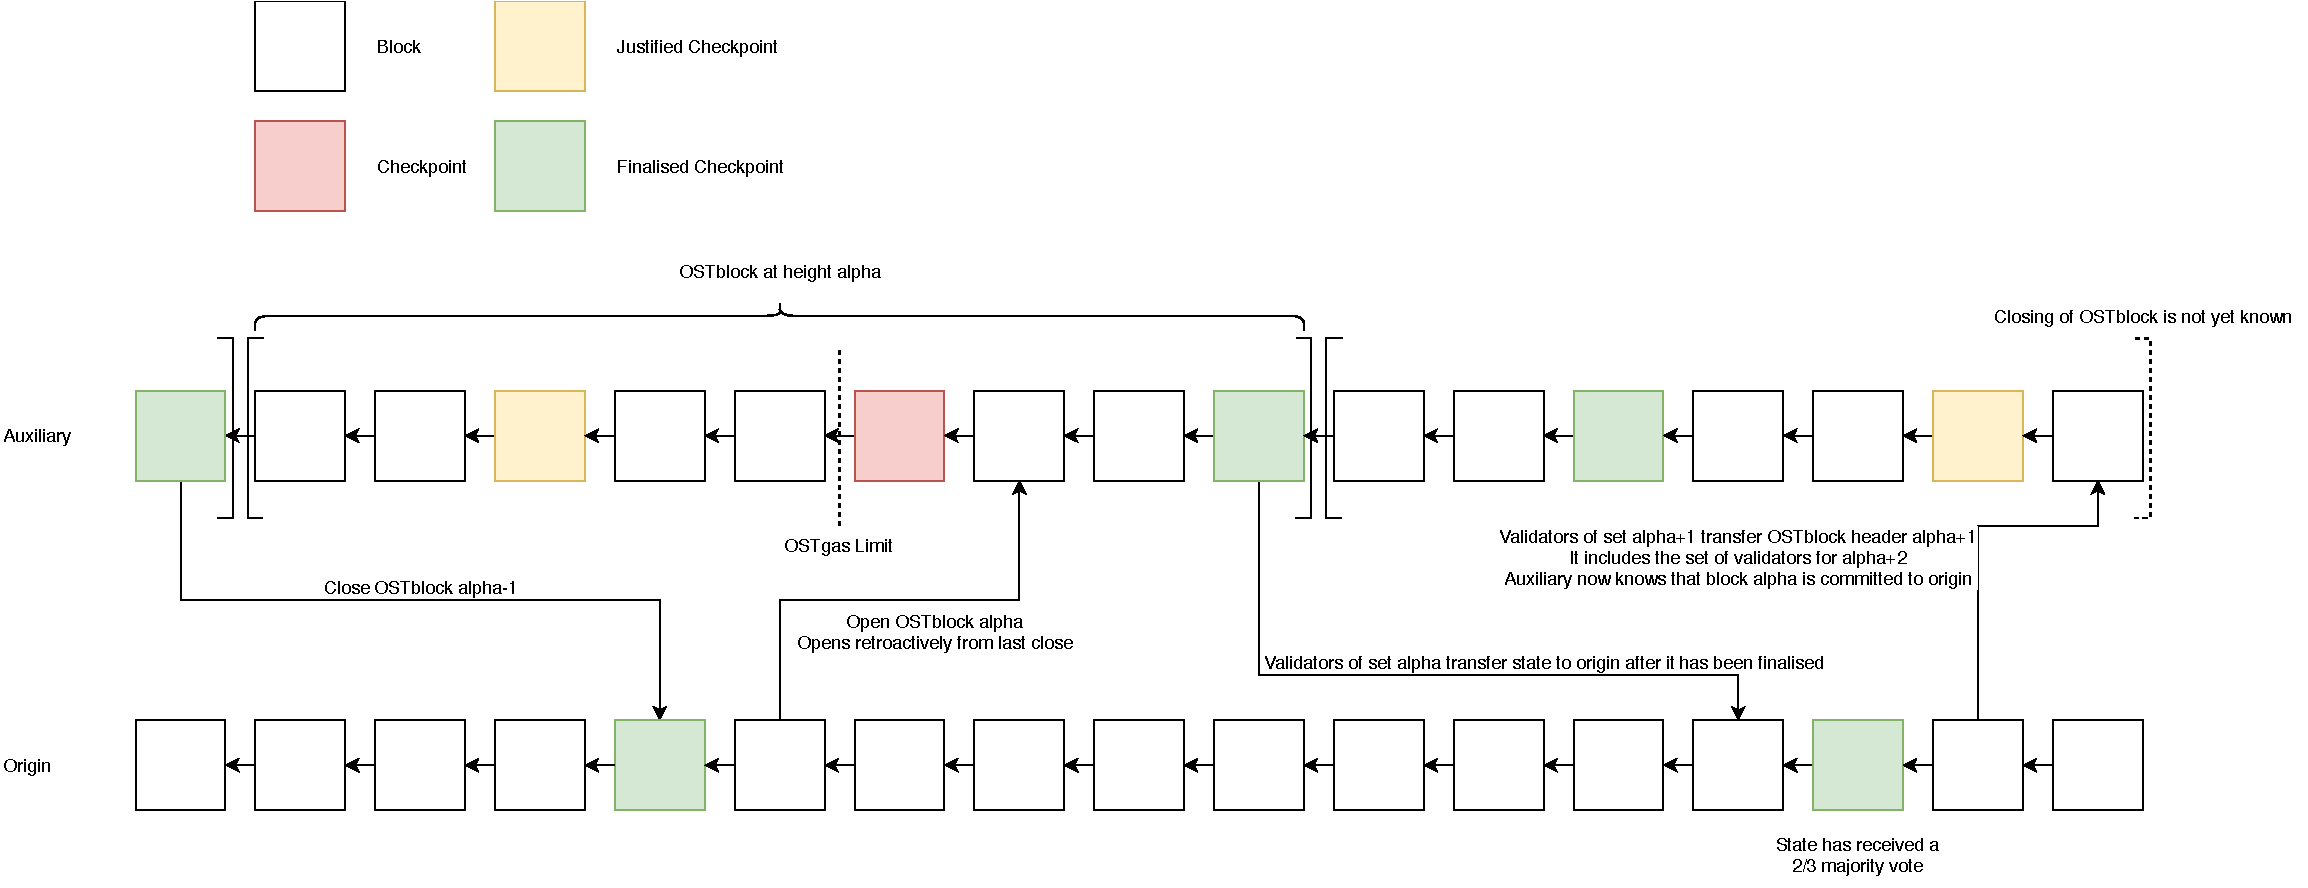
\includegraphics[width=\textwidth]{mosaic}
	\caption{The Mosaic State Transfer}
	\label{fig:mosaic}
\end{figure}
In order to be block proposal mechanism agnostic, we layer Casper~\cite{casperffg} on top of auxiliary.
% TODO missing context. Extend or move to validators paragraph above
Validators vote on supermajority links.
Auxiliary must follow Casper's fork choice rule.
%% TODO missing context
Checkpoints get finalised.
The validators can transfer the state of a finalised auxiliary checkpoint to origin.
% TODO language
A validator uses the Mosaic Gateway to transfer the state to origin.
On origin, a $\frac{2}{3	}$ majority vote is required by the validators in order to commit the state on origin.
The state is regarded economically finalised when the block that contains the commit is considered economically final on origin.

% TODO extend this paragraph
On the auxiliary chain, \emph{OSTgas} is the equivalent to gas on Ethereum.
For transactions to be included in blocks on auxiliary, a fee is paid for the consumed OSTgas.

Validators could commit every finalised state from auxiliary to origin.
However, that may be infeasible due to constraints on origin or from an economic viewpoint of the validators.
Therefore, we propose points in the life of the auxiliary chain where the validators must close the OSTblock.
% TODO link to figure; explain here or above where figure is explained; or move figure down
Whenever a certain, fixed limit of OSTgas has been spent on auxiliary since the opening of the OSTblock,
the validators must close the OSTblock at the next finalised auxiliary checkpoint. 

Actors on the auxiliary chain have an economic incentive to finalise their state on origin.
The block creators of auxiliary will pay a fraction of their earned OSTgas to the validators as a fee when the validators move the state to origin.
% TODO context and language
Due to the OSTblocks, validators can only copy the state from auxiliary to origin after the state of origin has been copied to auxiliary.
Thus, validators are incentivised to close an OSTblock and open a new one in order to earn the OSTgas fee for the transfer of auxiliary's state.

The set of validators needs to be able to change.
The logic is similar to that of Casper with the notable difference that, instead of dynasties, we use OSTblocks.
When a potential validator sends a \emph{deposit message} on origin at OSTblock height $\alpha$,
then the validator $\upnu$ will join the validator set at OSTblock height $\alpha+2$.
% TODO a lot copied from Casper. OK? Required?
Analogous to Casper, we call $\alpha+2$ the validator's \emph{start OSTblock}, $\BS(\upnu)$.
If a validator $\upnu$'s withdraw message is included on origin's blockchain during an open OSTblock $\B_\alpha$,
it similarly leaves the set of validators at OSTblock height $\alpha+2$.
We call $\alpha+2$ the validator $\upnu$'s \emph{end OSTblock} $\BE(\upnu)$.

% TODO Slashing validators on origin (e.g. when they misbehave on auxiliary)

% TODO Keeping stake four months back on origin should mean a shorter time back on auxiliary to forbid voting (3 months?)

%
% Section
%
\section{Securing Simple User Experience}

\subsection{Token Holder Contracts}

APIs; no need to follow the chain.

%
% Section
%
\section{Platform}

\subsection{Token Rules}

\subsection{OpenST Platform}

%
% Section
%
\section{Outlook}

\subsection{Neo and Cardano}

%
% Section
%
\section{Conclusion}

\bibliographystyle{naturemag}
\bibliography{openst}

\end{document}
